\chapter{脑机接口及相关信号}

\section{脑机接口简介}

由于现代计算机技术和神经科学学科的迅速发展,人们已经可以将大脑中的运动与计算机设备相关联,通过机器捕捉大脑中神经元的活动\cite{wolpaw2002brain}。这种为大脑和外部设备之间建立通路的方法与应用统称为脑机接口(brain computer interface,或BCI)\cite{van2009brain,donoghue2002connecting},以探索大脑活动与特定神经状态的关系。 脑机接口可以通过测量脑信号从而理解主体意愿, 而无需做出任何动作指示\cite{kostov2000parallel,allison2007brain,birbaumer2007brain}。 因此BCI对残障人士或运动皮层受损, 不能很好地与肌肉通信的病人有很大辅助作用。 比如对于脊侧索硬化\cite{allison2007brain}病人, 如果可以有效地对脑信号解码, 分析其意愿, 就可以通过外设完成相应操作, 从而辅助病人。 

现在有很多测量脑信号的技术,如fMRI (functional magnetic resonance imaging,功能性磁共振成像),NIRS(near-infrared spectroscopy,近红外光谱学),EEG(Electroencephalograph,脑电图),MEG(Magnetoencephalography,脑磁图)等。 针对不同的采集信号,其信号预处理方法也各不相同。但是BCI最基本的任务都是正确地识别次级类别并翻译成机器指令以完成用户的意愿。 脑机接口整个过程技术如图\ref{Fig:bci_brief}所示\cite{farwell1988talking},一个BCI需要包括:

\begin{enumerate}
\item{记录大脑活动}\\
	第一步, 需要用放大器采集脑信号。 
\item{提取并处理脑信号}\\
	第二步, 需要将脑信号进行预处理, 并分析其属于哪一类刺激, 即进行信号解码。 该步骤的解码部分非常重要, 包括脑信号特征提取并翻译的过程。 如果解码错误, 后面的两步就会变得无意义了。
\item{将脑信号翻译成计算机指令}\\
	第三步, 将解码后的信号发送到外部设备, 执行相关指令。
\item{最后返回给用户}\\
	最后, 外部设备将结果返回给用户。
\end{enumerate}

图\ref{Fig:bci_brief}中, 签名表示大脑神经信号的特定状态。 

\begin{figure}[htb]
\centering
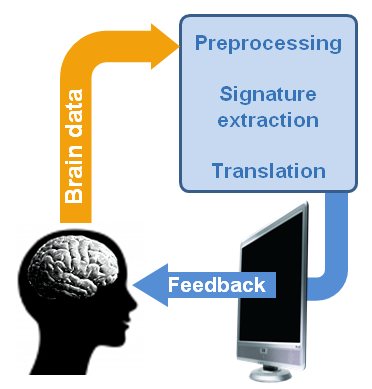
\includegraphics[scale=0.8]{Pictures/Chap1/bci_cycle_v2-2.png}
\caption{BCI 框架\cite{farwell1988talking}}
\label{Fig:bci_brief}
\end{figure}

在第二步的解码中, 采用一个信号分类器, 对不同刺激产生的信号进行分类。 已有很多方法针对信号解码提出一些的模式识别方法。 大多数有效方法基于机器学习模型\cite{blankertz2006berlin,lotte2007review,muller2008machine}, 如支持向量机(SVM)\cite{cortes1995support}, 隐马尔科夫模型(HMM)和神经网络模型都曾被用于神经解码。 此外, W.Wu等人基于卡尔曼滤波器建立了一个实时解码系统, 对运动皮层手臂区域大约40个神经元上所采集到的spike活动进行解码, 并证明其效果好于之前用到的线性滤波器技术\cite{wu2003neural}。 在根据神经信号进行手臂路径跟踪方面, Gyron M. Yu 在模型复杂度和分类效果上做了一个平衡, 提出了一个模型, 将一些简单轨迹模型结合到一个估计轨迹的概率混合模型中, 提高了分类准确率\cite{byron2007mixture}。 对于类似的手运动轨迹方向估计, Caleb Kemere等人基于学习的方法为运动轨迹建立了一个模型, 并用最大似然估计进行参数求解\cite{kemere2004model}。 T. Horikawa等人通过学习人在睡觉时候的fMRI与文字描述之间的联系进行神经信号解码\cite{horikawa2013neural}。 Lotte对基于EEG信号的脑机接口分类技术做了总结\cite{lotte2007review}。


\section{从视觉刺激到肌肉运动}

猴子对复杂的可视化刺激可以快速反应, 平均反应时间在250-260ms, 最短可以达到180ms。 因此在试验中, 我们建立了一套训练系统, 采集猕猴运动皮层的神经电信号。 如图\ref{Fig:brain_stimulate_flow}所示为一个基于视觉刺激, 从视网膜到肌肉执行操作的有可能的大脑通路图\cite{thorpe2001seeking}。 信息从视网膜传递到背外侧膝状体核(lateral geniculate necleus, LGN), 经过延迟传递到V1(主要的视觉皮层) 。 紧接着, 信息经过V2区,V4区,再到后、前颞皮质区(Inferotemporal cortex), 进行物体(高层)特征分析与描述。 后颞皮质将信息映射到不同区域,包括可以进行物体分类的前额皮质(prefrontal cortex cortex, PFC)。 为了将理解的命令传给肌肉执行, PFC又把信息通过运动前皮质区(premotor cortex, PMC)和运动皮层(motor cortex, MC)传递给脊髓的运动神经元。 最后,脊髓的运动神经元受刺激从而触发肌肉运动。 图\ref{Fig:brain_stimulate_flow}中, 每个信息处理过程后有一个以毫秒为单位的时间, 表示信息处理的估计时间, 这样的反应速度也决定了我们采集信号的频率。

\begin{figure}[htb]
\centering
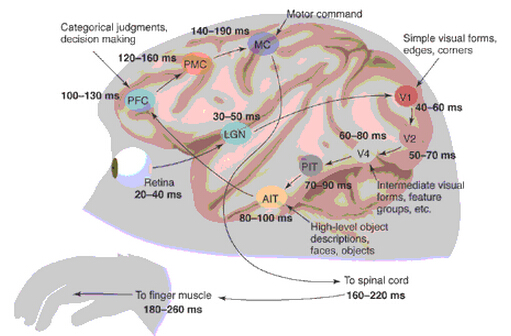
\includegraphics{Pictures/Introduction/brain_flow.jpg}
\caption{可视化刺激任务的大脑通路\cite{thorpe2001seeking}}
\label{Fig:brain_stimulate_flow}
\end{figure}



\section{P300信号检测}\label{sec:introduction_p300}

P300信号是人脑EEG信号中的波形, 受任务相关事件刺激而产生。 激发出P300信号的经典方法是通过“oddball task”产生, 即在一个任务中出现两种模式随机出现, 一种是频繁出现的, 另一种是很罕见的模式。 在任务中, 给定一个刺激,并指导试验个体给出刺激所属模式, 同时采集试验个体的EEG信号, 罕见模式出现时对应的脑信号为P300信号。 例如, 在字符拼写任务中, oddball task是一个关于字符注意的实验(如图\ref{Fig:P300_brief}\cite{polich2007updating}),展现一串字符(如SSTSSSSTSS),其中出现频率高的称为标准刺激(如该信号序列中的S),频率低的称为异常刺激(如该信号序列中的T)。当出现一个异常刺激时,300ms后就会在EEG信号中产生一个正向偏移点位。这里标准刺激和异常刺激的差异可以用来识别所给刺激的类别,然后基于刺激发送信号给计算机指令执行。
 
\begin{figure}[htb]
\centering
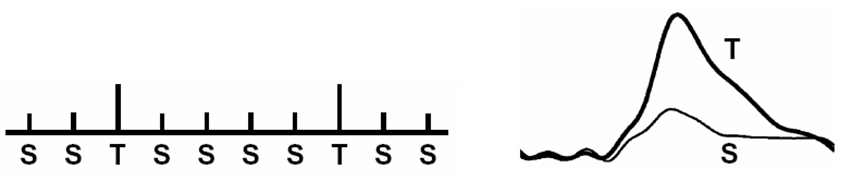
\includegraphics[scale=0.6]{Pictures/Chap1/p300_example.png}
\caption{P300刺激信号. 标准刺激(S)中的异常刺激(T)\cite{polich2007updating}}
\label{Fig:P300_brief}
\end{figure}


1988年 L. A. Farwell 和 E. Donchin 第一次用oddball task建立BCI系统\cite{farwell1988talking}。 该系统中,将36个字符展现在一个6*6的矩阵中, 矩阵的行和列随机闪烁, 同一时刻只有一行或一列亮起,具体哪一行或哪一列是随机的。 如图\ref{Fig:p300matrix}所示, 当一行一列相继闪烁的交点为指定字母时, 测试者可以集中精神在头脑中进行简单计数或者确认, 相应就会有P300在该位置产生, 可以通过估计算法检测到这个P300信号。 也就是说, 如果在对应字母闪烁300ms后在某个位置检测到了P300信号, 就说明主体正在注意这个特定位置。 所以P300的检测实际上就是主体关注位置点字符的检测。  

\begin{figure}[htb]
\centering
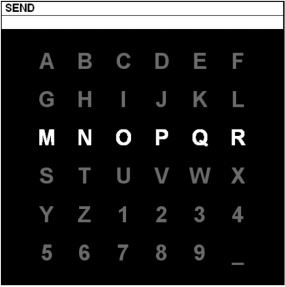
\includegraphics[scale=0.8]{Pictures/Chap1/p300_matrix.jpg}
\caption{oddball task实验矩阵\cite{cecotti2011convolutional}}
\label{Fig:p300matrix}
\end{figure}

在P300检测中, 需要先后两个过程。 第一步, P300位置检测。 这是一个二类分类问题, 给定一个时间段的信号, 判断是否为P300波形。 这个是在实验中进行标注的。 比如, 主体确定了当前要关注的字符, 给定固定顺序随即闪烁行列的矩阵, 我们就可以根据闪烁次序知道当前是否闪烁指定字符, 即是否预期产生P300波形。 但由于一些人为因素干扰, 测试主体不一定能在指定时刻真的给出P300响应, 所以第一步的目标是对这个带噪声的数据进行分类。 第二步根据第一步的分类结果, 对是P300的信号分类属于36个字符中的哪一个。


\section{研究问题与目标}

本文中, 我们将分别用到两种BCI采集到的信号。 脑机接口可以分为侵入式和非侵入式,非侵入式方法,如头皮电信号(scalp electroencephalogram,EEG)易于获取,但是信号精度很差,采样率也相应很低。相反,侵入式脑机接口用外科手术的方法将电极植入大脑皮层进行信号采集,可以采集到很高精度的细胞外神经元信号。在单个神经元中这种高精度信号包含神经锋电位(spike),或者叫做动作电位(action potential)。当神经元被激发的时候就会在神经元膜上产生离子电流,导致细胞去极化(depolarize)并激发出一个spike信号。

本文的研究内容主要有, 侵入式脑机接口的信号压缩, 以及非侵入式脑机接口的信号解码中的一种任务——P300信号检测。 对于侵入式脑机接口, 有信号采集难, 信号采样率高的问题, 导致传输与存储困难。 已有一些工作关注非侵入式脑机信号的采集压缩, 如Electromyography(EMG)和Electroencephalography(EEG)信号的压缩\cite{24,25},为了有效压缩,他们都结合了所处理信号的信号特性, 但是侵入式胞外信号与之相差甚远。 原因是非侵入式信号采集自头皮, 有效信号只在低频部分, 所以可以通过在频域低通滤波进行很大程度上的信号压缩, 但侵入式信号中含有高频spike信号, 难以简单过滤, 使该任务更富有挑战性。 Chen等人对老鼠的S1区域进行研究,通过自适应信号量化在信噪比保持25db的时候达到的压缩率高于25\%,那么信号压缩率和信号质量都得不到保证。 本文中, 我们在浙江大学求是学院BCI系统 \cite{14}上进行植入式运动皮层信号的信号压缩。

对于非侵入式脑机接口, 已有很多相关工作在P300检测方面进行研究, 包括基于SVM\cite{rakotomamonjy2008bci}, LDA\cite{breiman1996bagging}, ICA\cite{yang2008p300}和卷积神经网络\cite{felzer2003analyzing,anderson1995determining,cecotti2008time,masic1995neural,masic1993neural}的方法等。 近年来, 深度学习方法凭借可训特征(或可训的kernel)优势,在语音识别, 图像处理, 声音合成, 生物信号分析等方面超过了手工定义特征的传统方法, 借助现代计算机计算能力的提高和大数据量的爆发得以广泛应用。 本文中, 也采用深度学习的方法进行EEG信号建模, 提高其对P300波形检测效果。 这里我们采用两种模型: 卷积神经网络和循环神经网络模型。 对于卷积神经网络, 已有相关工作进行建模并达到较好的P300检测效果, 但在其模型中有很多部分可以进行改进。 在我们的ConvP300Net方法中, 通过改进模型结构, 可以更好地利用信号空间相关性; 通过重新设计对数据不均衡问题的处理方法, 可以使模型更好地拟合所用数据, 而不需考虑模型集成问题带来的识别增益; 此外ConvP300Net中还加入了很多模型调整部分与方法优化。 对于循环神经网络, 目前很少有方法对非侵入式信号进行处理, 但我们注意到循环神经网络, 尤其是其中的长短时间记忆方法, 可以很好地利用时间维度相关性对时间序列进行建模, 同时避免了传统循环神经网络训练难以收敛的问题。 因此, 本文中设计了LSTMP300Net, 采用长短时间记忆方法对EEG信号建模 , 使其能够更好地拟合信号在P300检测任务上的信号特性。 


之所以分别对侵入式脑机信号和非侵入式脑机信号进行不同任务(压缩和解码), 主要是为了提高问题难度。 侵入式脑机信号难以有效压缩, 且信号采集难度大,对平台有要求,有一些工作分别结合自己的BCI平台进行侵入式脑机接口压缩, 但非常依赖所采集的信号;  非侵入式脑机信号噪声大, 难以进行信号解码, 已有很多工作结合机器学习提出了非侵入式脑机接口神经解码方法, 深度学习的方法虽然在其中占比不高, 但可与一些已有工作进行比较。 所以我们分别在这两种数据上进行信号压缩与解码, 提高研究问题的挑战性。 


本文的目标是, 在侵入式脑机信号的压缩方面, 在保证信号重建质量的基础上提高压缩性能, 使之超过传统数据/文档压缩方法; 在非侵入式脑机信号的P300波形监测方面, 分别采用ConvP300Net和LSTMP300Net超过已有基于神经网络的检测方法。  对于ConvP300Net, 我们在已有相关工作上进行改进, 着重考虑模型调整, 更好地利用信号在空间维度的相关性以及如何直接在网络中考虑各类样本数差异所带来的数据非均匀问题。 对于LSTMP300Net, 我们基于长短时间记忆方法提出了该模型, 并调整网络结构以得到最佳P300波形检测效果。



\section{文章结构}

本文的组织结构如下: 在第二章中, 我们针对侵入式神经信号占用空间大, 传输困难的问题对其进行压缩, 提出了一个新颖的压缩框架, 并在猕猴上采集的神经电信号数据上证明了其有效性。 之后, 我们在非侵入式EEG信号上采用深度学习的方法进行P300检测中的第一个环节,即 检测一段信号是否是P300信号。 第三章和第四章分别采用卷积神经网络和循环神经网络对其进行建模, 构建了ConvP300Net和LSTMP300Net并分析模型的有效性。 这里之所以在压缩部分采用侵入式脑机接口所得神经电信号是因为项目平台需要。 侵入式神经电信号的高精度高采样率决定了其大数据量, 阻碍了在我们的信号采集平台中的快速传输, 需要对其压缩, 而现有神经信号压缩方法都会使信号失真, 所以需要针对我们所采集的信号特性进行高保真神经电信号压缩。 而第三、四章在神经解码应用中我们采用的是非侵入式方法所得的EEG信号, 这是出于方便与其他模型比较考虑的。 在三、四章中, 我们采用公开BCI竞赛数据集\cite{blankertz2006bci}, 已有很多包括神经网络在内的方法应用于该数据集以提高神经信号解码效果, 采用该数据集方便我们进行合理的模型比较, 而据我们所知, 侵入式脑电信号没有公开竞赛数据集。









